\begin{figure*}[!t]
    \centering
    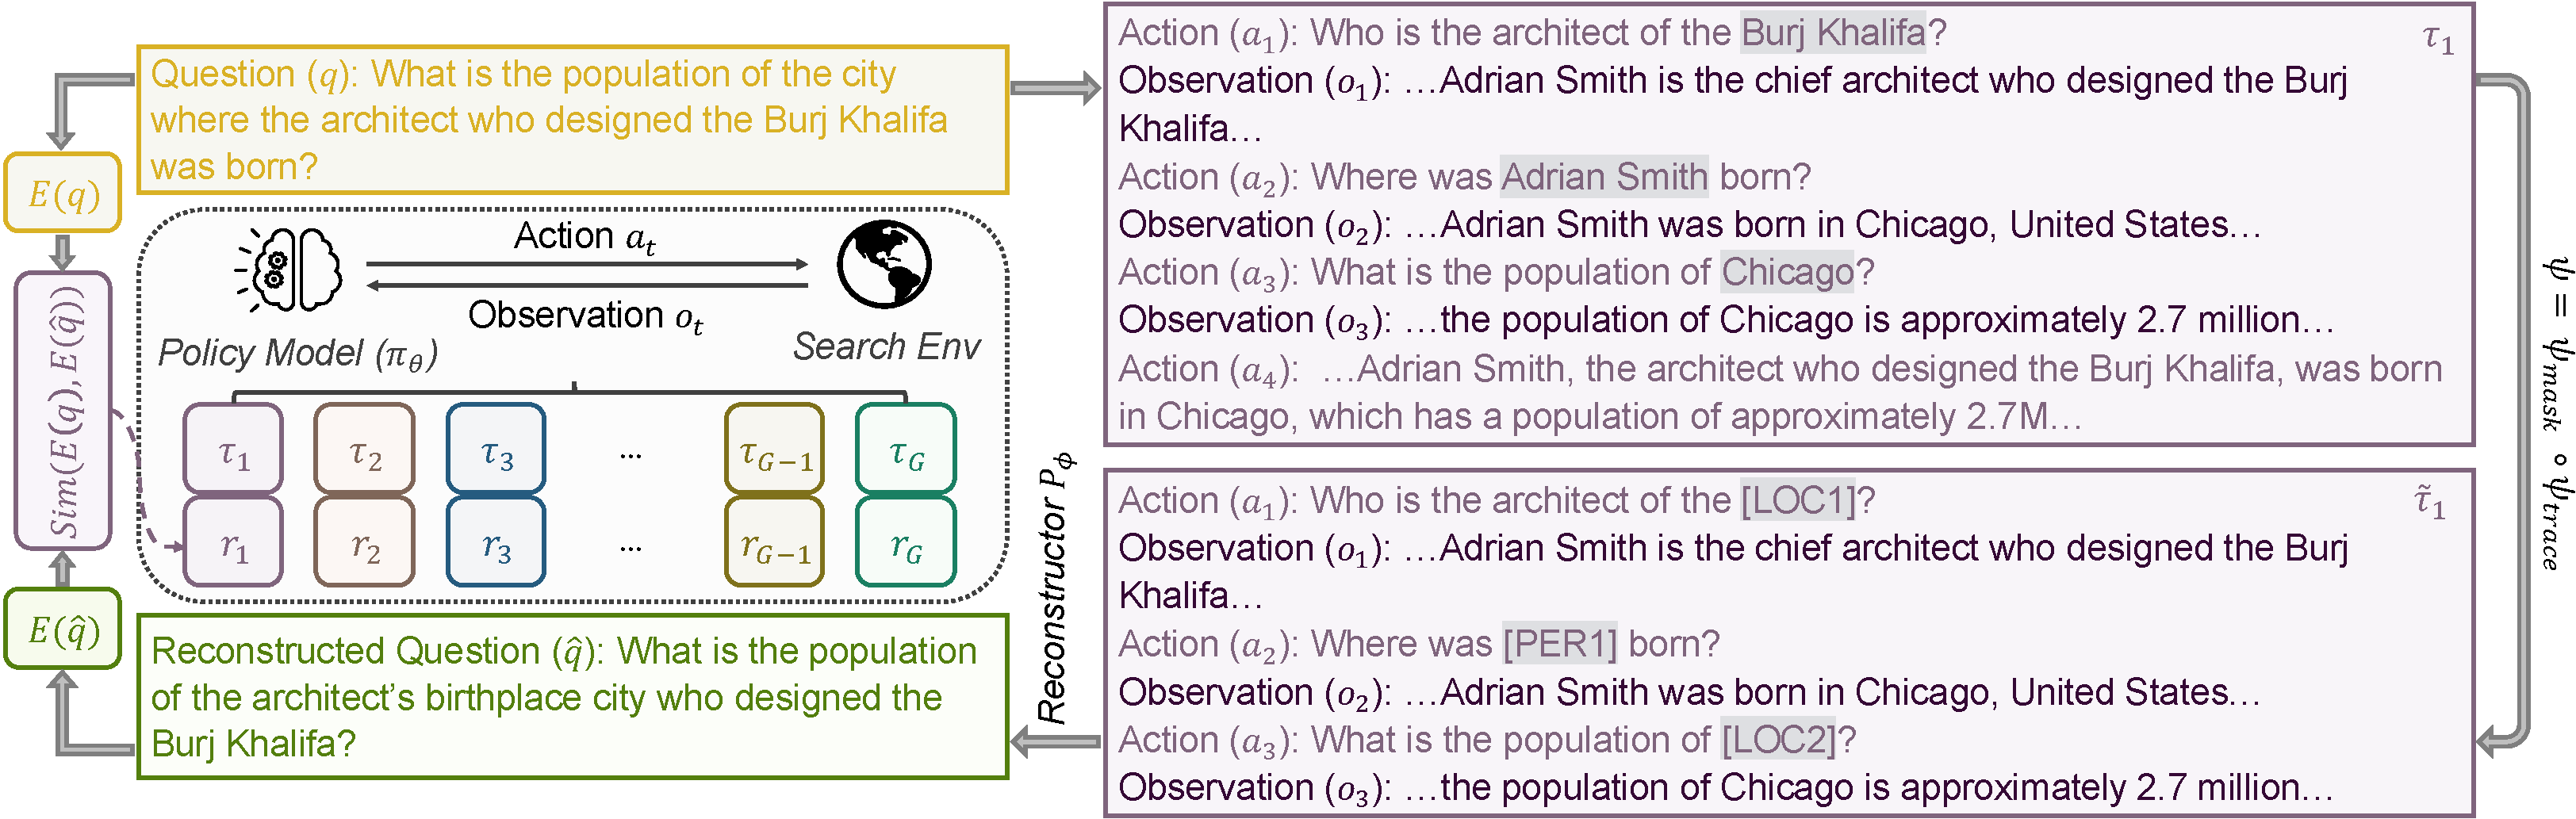
\includegraphics[width=1\linewidth]{img/ccs_main.pdf}
    \caption{\textbf{Overview of the Cycle-Consistent Search (CCS) framework.} The agent $\pi_\theta$ generates search trajectories $\tau$ to address a question $q$. To ensure the search process is driven by information gain rather than lexical copying, $\tau$ is passed through a strategic information bottleneck ($\psi$) that removes the $a_T$ and masks entities within actions (highlighted in grey). A frozen reconstructor $P_\phi$ then attempts to recover the original question from $\tilde{\tau}$. The agent is optimized using GRPO based on the semantic similarity between $q$ and $\hat{q}$, encouraging trajectories that capture sufficient evidence.}
    \label{fig:ccs_main}
\end{figure*}